\documentclass[showpacs,preprintnumbers,amsmath,amssymb,superscriptaddress,aip]{revtex4-1}
\usepackage{graphicx}
%\setlength{\parindent}{0in}

% General Latex  --------------------------------------------------
\def\beq{\begin{equation}}
\def\eeq{\end{equation}}
\def\beqar{\begin{eqnarray}}
\def\eeqar{\end{eqnarray}}
\def\nn{\nonumber}
\def\ol{\overline}
\def\para{\parallel}

% Operators  ------------------------------------------------------
\newcommand{\diff}[2]{\frac{d#1}{d#2}}
\newcommand{\diffs}[2]{\frac{d^2#1}{d#2^2}}
\newcommand{\pdiff}[2]{\frac{\partial#1}{\partial#2}}
\newcommand{\pdiffs}[2]{\frac{\partial^2#1}{\partial#2^2}}
\newcommand{\pdiffxy}[3]{\frac{\partial^2#1}{\partial#2 \partial#3}}
\newcommand{\pdt}{\partial_t}
\newcommand{\pdr}{\partial_r}
\newcommand{\pdth}{\partial_\theta}
\newcommand{\pdrr}{\partial^2_r}

\newcommand{\enum}[2]{{#1}\times10^{#2}} % 4.2x10^{3} = \enum{4.2}{3}

\newcommand{\vect}[1]{{\bf #1}}
%\newcommand{\vect}{\overrightarrow}
%\newcommand{\vect}{\vec}
\def\div{\nabla\cdot}
\def\grad{\nabla}
\def\curl{\nabla\times}
\newcommand{\gradpar}{\grad_\parallel}
\newcommand{\gradperp}{\grad_\perp}
\newcommand{\gradr}{\grad_r}
\newcommand{\defeq}{\ensuremath{\stackrel{\text{\tiny def}}{=}}}

\newcommand{\savg}[1]{\left<{#1}\right>}
\newcommand{\vavg}[1]{\left<{#1}\right>_V}
\newcommand{\thavg}[1]{\left<{#1}\right>_\theta}

% Variable names  -------------------------------------------------
\newcommand{\vpar} {v_\parallel}
\newcommand{\Apar} {A_\parallel}
\newcommand{\jpar} {j_\parallel}
\newcommand{\kpar} {k_\parallel}
\newcommand{\kperp} {k_\perp }
\newcommand{\vperp} {v_\perp }
\newcommand{\kthe}{k_\theta}

\newcommand{\Evec}{\ensuremath{\boldsymbol{{\rm E}}}}
\newcommand{\Bvec}{\ensuremath{\boldsymbol{{\rm B}}}}
\newcommand{\Jvec}{\ensuremath{\boldsymbol{{\rm J}}}}
\newcommand{\Fvec}{\ensuremath{\boldsymbol{{\rm F}}}}
\newcommand{\fvec}{\ensuremath{\boldsymbol{{\rm f}}}}
\newcommand{\vE}{\ensuremath{\boldsymbol{{\rm v}_{E}}}}
\newcommand{\bo}{\ensuremath{\boldsymbol{{\rm b}_0}}}
\newcommand{\bvec}{\ensuremath{\boldsymbol{{\rm b}}}}
\newcommand{\xvec}{\ensuremath{\boldsymbol{{\rm x}}}}
\newcommand{\yvec}{\ensuremath{\boldsymbol{{\rm y}}}}
\newcommand{\zvec}{\ensuremath{\boldsymbol{{\rm z}}}}
\newcommand{\vvec}{\ensuremath{\boldsymbol{{\rm v}}}}
\newcommand{\jvec}{\ensuremath{\boldsymbol{{\rm j}}}}

\newcommand{\bxgp}{\bvec\times\gradperp}

\newcommand{\vve}{\ensuremath{\boldsymbol{{\rm v}}_{e}}}
\newcommand{\vvi}{\ensuremath{\boldsymbol{{\rm v}}_{i}}}
\newcommand{\vpe}{v_{\parallel e}}
\newcommand{\vpi}{v_{\parallel i}}
\newcommand{\vvE}{\ensuremath{\boldsymbol{{\rm v}}_{E}}}
\newcommand{\vvD}{\ensuremath{\boldsymbol{{\rm v}}_{D}}}

\newcommand{\nuei}{\nu_{ei}}
\newcommand{\nuii}{\nu_{ii}}
\newcommand{\nue}{\nu_{e}}
\newcommand{\nuen}{\nu_{en}}
\newcommand{\nuin}{\nu_{in}}
\newcommand{\kpe}{\kappa_{\parallel e}}

\newcommand{\rs}{\rho_{s}}
\newcommand{\ri}{\rho_{i}}
\newcommand{\wci}{\Omega_{i}}
\newcommand{\wcix}{\Omega_{ix}}
\newcommand{\wce}{\Omega_{e}}
\newcommand{\tomega}{\tilde\omega}
\newcommand{\Isat}{I_{\rm sat}}
\newcommand{\fmie}{\frac{m_i}{m_e}}
\newcommand{\fmei}{\frac{m_e}{m_i}}


% Often used dimensions
\newcommand{\cm}{\rm cm}
\newcommand{\mm}{\rm mm}
\newcommand{\cmn}{{\rm cm}^{-3}}
\newcommand{\mn}{{\rm m}^{-3}}
\newcommand{\eV}{\rm eV}
\newcommand{\G}{\rm G}
\newcommand{\T}{\rm T}



\begin{document}

\title{Non-modal Growth in LAPD Turbulence}

\author{B. Friedman}
\email{friedman@physics.ucla.edu}

\author{T.A. Carter}

\affiliation{Department of Physics and Astronomy, University of California, Los Angeles, California 90095-1547, USA}



\begin{abstract}
Large Plasma Device (LAPD) [W. Gekelman \emph{et al.}, Rev. Sci. Inst. {\bf 62}, 2875 (1991)] 
\end{abstract}

\maketitle

\section{Introduction}

Normal mode analysis -- dealing with the eigenvalues and eigenvectors of a dynamical system -- has been used for the last two centuries to solve a number of problems ranging from
heat conduction along a solid bar to quantum mechanical energy states of atoms. Despite its wide-ranging success, normal mode analysis has seemingly failed in particular instances,
particularly in predicting the onset of turbulence in many hydrodynamic flows, where the turbulence is called subcritical. 
The reason for this failure was not clearly explained until the early 1990's when Trefethen and others attributed the pitfalls of normal mode analysis to the non-normality of
systems~\cite{trefethen1993,trefethen2005} -- a non-normal system is one whose linear matrix or operator does not commute with its adjoint. 
Non-normal systems have eigenvectors that are nonorthogonal to one another. One consequence of non-normality is that even when all of the eigenvalues lie in the stable domain 
(where all linear eigenvectors decay exponential), some fluctuations can transiently grow by accessing the free energy in the equilibrium gradients, allowing for sustained turbulence. 
A paradigmatic illustration of this transient growth process for two nonorthogonal eigenvectors may be seen if Figure 2 of a review paper by Schmid~\cite{schmid2007}.
Such behavior is obscured by traditional normal mode analysis, which only effectively describes the long time asymptotic behavior of fluctuations under the 
action of the linear operator. Transient events, such as those that can dominate nonlinear turbulent evolution, require initial-value (non-modal) calculations rather than normal mode calculations.

Non-modal analysis has been embraced by the hydrodynamics community over the past two decades in the attempt to explain and predict subcritical turbulence, but the plasma community
still heavily relies on normal mode analysis to inform turbulent predictions and observations, with a few notable exceptions~\cite{camargo1998,camporeale2010,schekochihin2012}. 
Additionally, non-modal treatments thus far have generally been used to explain rather than predict turbulent characteristics, 
while the few predictions that have been made are often qualitative rather than quantitative. Perhaps this is why non-modal analysis has not received greater attention.
Therefore, this paper takes up the task of developing a quantitative approach to predicting turbulent properties using only non-modal linear calculations. 
The basic approach we take is to solve the linear initial value problem using an ensemble of random initial conditions, 
and then calculate the average growth rate of the solutions up to one nonlinear decorrelation time, which we take to be the characteristic time of the linear process. 
The effective growth rate spectrum produced by this technique can then be used in a quasilinear fashion to gain more information about the turbulence.
While this technique is general and can be applied to many nonlinear dynamical systems, we restrict our treatment to one particular model that relates to one particular experiment. Not only does
this allow us to thoroughly explain and validate this technique, but it also allows us to attribute transient growth effects to physically realizable turbulence.

The experiment considered is a drift wave turbulence experiment conducted in the Large Plasma Device (LAPD)~\cite{gekelman1991}. LAPD is a linear machine with a straight magnetic field $\mathbf{B}$.
Due to its large dimensions and high collisionality, LAPD is suitable for fluid modelling. We use a reduced Braginskii~\cite{Braginskii1965} 2-fluid model:

\beqar
\label{ni_eq}
\pdt N = - {\mathbf v_E} \cdot \grad N_0 - N_0 \gradpar \vpe + \mu_N \gradperp^2 N + S_N + \{\phi,N\}, \\
\label{ve_eq}
\pdt \vpe = - \fmie \frac{T_{e0}}{N_0} \gradpar N - 1.71 \fmie \gradpar T_e  + \fmie \gradpar \phi - \nue \vpe + \{\phi,\vpe \}, \\
\label{rho_eq}
\pdt \varpi = - N_0 \gradpar \vpe  - \nuin \varpi + \mu_\phi \gradperp^2 \varpi + \{\phi,\varpi \}, \\
\label{te_eq}
\pdt T_e = - {\mathbf v_E} \cdot \grad T_{e0} - 1.71 \frac{2}{3} T_{e0} \gradpar \vpe + \frac{2}{3 N_0} \kpe \gradpar^2 T_e  \nonumber \\
- \frac{2 m_e}{m_i} \nue T_e  + \mu_T \gradperp^2 T_e +  S_T + \{\phi,T_e\},
\eeqar
where $N_0$ and $N$ are the equilibrium and fluctuating density, $\vpe$ is the fluctuating parallel electron velocity, $\varpi \equiv \gradperp \cdot (N_0 \gradperp \phi)$ is the potential vorticity
of the fluctuating potential $\phi$, and $T_{e0}$ and $T_e$ are the equilibrium and fluctuating electron temperature. The equations are developed with Bohm normalizations: lengths are
normalized to the ion sound gyroradius $\rho_s$, times to the ion cyclotron time $\omega_{ci}^{-1}$, velocities to the sound speed $c_s$, densities to the equilibrium peak density, and electron
temperatures and potentials to the equilibrium peak electron temperature. The profiles $N_0$ and $T_{e0}$ and other parameters are all taken from experimental measurements. Note that $\phi_0$ is
neglected because we model only one experiment in which the equilibrium radial electric field was nulled out by boundary biasing~\cite{schaffner2012}. 

The equations are global and partially linearized -- the only nonlinearities we retain are the advective nonlinearities in the Poisson brackets. 
We also add artificial diffusion and viscosity terms with small numerical coefficients ($\mu_N, \mu_\phi, \mu_T = 10^{-3}$), 
used for numerical stability in nonlinear simulations, which are performed with the BOUT++ code~\cite{dudson2009}. We use periodic axial and zero value radial 
boundary conditions. Further details of the model, including validation studies, may be found in the references~\cite{Popovich2010a,Popovich2010b,Umansky2011,friedman2012b,friedman2013},
though we mention here that the model reproduces all statistical properties of the experimental turbulence within a factor of two, and in most cases, much better than that.
Of particular interest, was the finding that the sustainment of the turbulence in the nonlinear simulation is dominated by a nonlinear instability process~\cite{friedman2012b,friedman2013}.
This nonlinear instability process -- discovered by Drake et al.~\cite{drake1995} in simulations using a similar plasma model to ours -- works as follows: long $k_\para=0$ convective filaments transport
density (and temperature to a lesser extent) across the equilibrium density profile, setting up $k_\para=0$ density filaments. These filaments are unstable to drift waves causing a secondary drift
wave instability to grow on the filaments. These drift waves, which have finite $k_\para$ and propagate primarily radially, nonlinearly couple to one another and reinforce the convective filaments.

\begin{figure}
\centerline{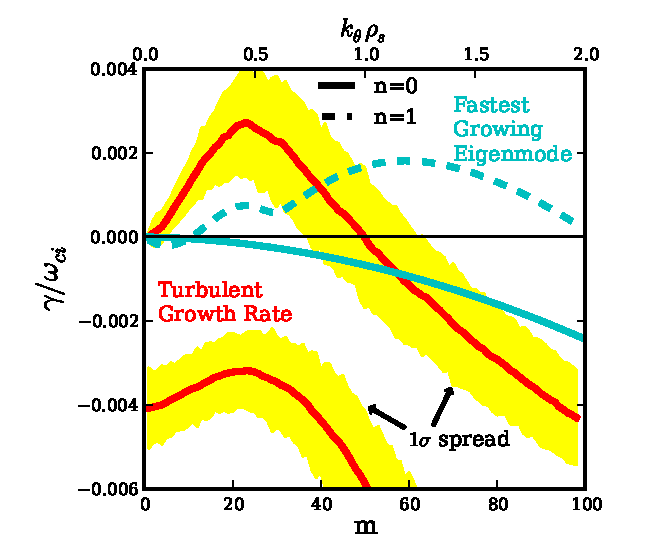
\includegraphics[]{spec_nl_gamma}}
\caption{The linear and turbulent growth rate $m$ spectra for $n=0$ (solid lines) and $n=1$ (dashed lines) Fourier components. The linear growth rates are those for the least stable eigenmodes at each
$n$ and $m$, while the turbulent growth rates represent $\pdiff{E}{t}|_{\rm{lin}}/2 E$ from the nonlinear simulation. The shaded region marks the $1 \sigma$ spread in the turbulent growth rate spectrum,
obtained from the distribution of growth rates calculated from the nonlinear simulation over a long time range.}
\label{spec_nl_gamma}
\end{figure}

Although the instability mechanism is nonlinear, the first part of the mechanism -- the transport of density by the convective filaments -- is a linear one. 
In fact, it is surprisingly similar to the so-called "lift-up'' mechanism often seen in subcritical hydrodynamic shear flows, for which transient growth arguments were first applied~\cite{trefethen1993},
making it particularly apt to explore in a non-modal framework. Furthermore, since the other steps of the nonlinear instability
are controlled by nonlinear interactions, the convective transport is the only step responsible for energy injection and dissipation from the laminar state. This fact may be seen from simple
energetic principles. Starting from Eqs.~\ref{ni_eq}-\ref{te_eq},
an equation for the evolution of the energy can be obtained~\cite{friedman2012b,friedman2013}. The equation takes the form:

\beq
\label{dEdt_def}
\diff{E(m,n,t)}{t} = Q(m,n,t) + D(m,n,t) + \sum_{m',n'} T(m,m',n,n',t).
\eeq
Here, $m$ and $n$ are the azimuthal and axial Fourier mode numbers, respectively. Note that since Eqs.~\ref{ni_eq}-\ref{te_eq} are not explicitly dependent on $\theta$ and $z$, the energy equation
is separable for every $m$ and $n$. Furthermore, $Q$ represents the linear energy exchange with the equilibrium, $D$ is the dissipation from irreversible processes
like collisions, and $T$ accounts for the nonlinear triad wave transfer. Because $T$ results from the Poisson bracketed advective nonlinearities in the model and $\int f \{g,f\} dV = 0$, 
$\sum_{m,m',n,n'} T(m,m',n,n',t)=0$, meaning the nonlinearities cause no net energy injection or dissipation. In other words, the fluctuation energy originates completely from the linear terms.

The expression $\diff{E(m,n,t)}{t}\big|_{\rm{lin}} = Q(m,n,t) + D(m,n,t)$ accounts for the total net energy injection at each $m,n$ into the fluctuations. 
An effective instantaneous growth rate $\gamma_{\rm{eff}}(m,n,t) = \diff{E(m,n,t)}{t}\bigg|_{\rm{lin}}/ 2 E(m,n,t)$ can then be defined. 
This effective growth rate is calculated from the spatial structure of the fluctuations, so it has meaning for turbulent fluctuations as well as those obtained from a linear simulation. If calculated
from a linear simulation run for a sufficiently long time, $\gamma_{\rm{eff}}(m,n)$ is the same as the eigenmode growth rate of the least stable linear eigenmode for each $m,n$.
We plot this effective growth rate in Fig.~\ref{spec_nl_gamma} for $n=0$ and $n=1$ components. The turbulent growth rate curves are calculated from this formula, 
averaged over a time of about $3 \times 10^{4} \omega_{ci}^{-1}$ during the saturated turbulent phase of the nonlinear simulation --$\gamma_{\rm{Turb}}(m,n) = \int \gamma_{\rm{eff}}(m,n,t) dt$. 
We show this turbulent growth rate along with the $1 \sigma$ contour, which indicates how greatly $\gamma_{\rm{eff}}(m,n,t)$ varies over time.
Along with these, the growth rates of the least stable (or most unstable) linear eigenmodes are shown.

From Fig.~\ref{spec_nl_gamma}, one sees that the linear eigenmodes are unstable for $n=1$ and stable for $n=0$ as expected for drift waves. 
However, the turbulent growth rates are positive for $n=0$ and low $m$, but negative for $n=1$ at all $m$. 
The net injection of the $n=0$ components is reminiscent of subcritical turbulence, where there is turbulent sustainment in the absense of linear instability.
Moreover, the $n=0$ energy injection is a manifestation of the convective filaments drawing energy from the equilibrium density gradient and depositing this energy into the density fluctuations,
which again, is similar to the hydrodynamic ``lift-up'' mechanism associated with subcritical hydrodynamic shear-flow turbulence.
It it prudent then to call the turbulence in the LAPD simulation subcritical or at least subcritical-like. 

Like subcritical hydrodynamic turbulence, the cause of subcritical LAPD turbulence (the positive growth rate of the $n=0$ structures) 
is a transient growth mechanism due to nonorthogonal linear eigenmodes. The transient growth can be seen clearly in Fig.~\ref{transient_n0_n1_growth},
where we follow the evolution of the energy of several Fourier $m,n$ modes after turning off the nonlinearities in the turbulent simulation. The $n=0$ modes grow for some time before decaying
exponentially at the rate of their least stable eigenmode. Conversely, the $n=1,m=20$ mode decays transiently before growing exponentially. This is not an attribute of subcritical turbulence
because there are no unstable eigenmodes in truly subcritical turbulence, but it is nevertheless interesting and is associated with a transient event.
The growth (or decay) rate of these curves at $t=0$ is necessarily equal to the growth rate that is used in the calculation of Fig.~\ref{spec_nl_gamma}. 
This $t=0$ growth rate, however, is just one number that goes into that calculation. The calculation is based on the turbulence over a long time range; this is just one instant of time.
In any case, the $t=0$ behavior of the curves in Fig.~\ref{transient_n0_n1_growth} generally corroborates with the effective growth rates in Fig.~\ref{spec_nl_gamma}.

\begin{figure}
\centerline{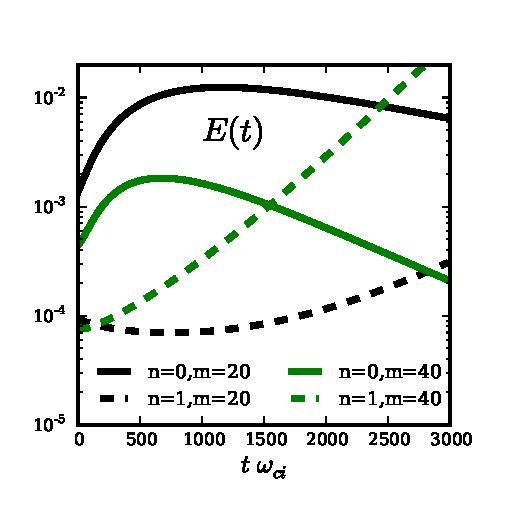
\includegraphics[]{transient_n0_n1_growth}}
\caption{The linear evolution of the energy of several Fourier modes starting from a turbulent initial state. The $n=0$ curves have an initial period of transient growth before exponentially decaying,
while the $n=1,m=20$ curve transiently decays before growing exponentially.}
\label{transient_n0_n1_growth}
\end{figure}

We stress again that Fig.~\ref{transient_n0_n1_growth} is obtained by \emph{linear} evolution from an initial turbulent state.
Since the transient growth (and decay) is a purely linear phenomenon, it appears possible to predict turbulent growth rates like those of Fig.~\ref{spec_nl_gamma} using only linear calculations.
Such calculations would be much faster and easier to interpret than direct simulations of nonlinear equations. However, the difficulty in such calculations lies in the dependence of the transient
evolution on the initial conditions and the change in the growth rate as a function of time as the linear evolution progresses. To overcome this difficulty, we propose a statistical procedure
that linearly evolves an ensemble of random initial conditions and calculates the average growth rate of the evolution over a characteristic linear time.

To elucidate this procedure, we take Eqs.~\ref{ni_eq}-\ref{te_eq}, remove the nonlinearities and sources and Fourier decompose in the azimuthal and axial directions.
Then, we discritize in the radial direction ($r \rightarrow r_0, r_1, \ldots, r_N $), and approximate radial derivatives with finite differences. 
The resulting system of equations may be written in matrix form:

\beq
\label{lin_eq}
\mathbf{B}_{m,n} \diff{\mathbf{v}_{m,n}(t)}{t} = \mathbf{C}_{m,n} \mathbf{v}_{m,n}(t),
\eeq
where $\mathbf{v}_{m,n} = \left( N(r_0), N(r_1), \ldots, \vpe(r_0), \vpe(r_1), \ldots, \phi(r_0), \phi(r_1), \ldots, T_e(r_0), T_e(r_1), \ldots \right)_{m,n}^{T}$,
and $\mathbf{B}_{m,n}$ and $\mathbf{C}_{m,n}$ are coefficient matrices that include the equilibrium information and finite difference coefficients. 
The equations for different $m$ and $n$ are separable because the equations are linear and the eigenfunctions have azimuthal and axial Fourier dependence resulting from the lack of explicit
dependence on $\theta$ and $z$ in the equations. Thus, eigenmodes with different $m$ and $n$ are orthogonal and linearly non-interacting. Note that for each $m,n$, there exist $4 \times N_r$ linearly
independent, but nonorthogonal eigenvectors. Hence forth, we drop the $m,n$ subscripts.

In order to use non-modal analysis to calculate growth rates and other measures, one must choose a norm and inner product with which to work. While any choice of
inner product is possible, including that which orthogonalizes all eigenvectors, a physically relevant one is generally preferred~\cite{camargo1998,schmid2007,camporeale2010}. The most commonly used
is an energy inner product. Recall that the inner product of two vectors may be written $\left< \mathbf{x},\mathbf{y} \right> = \mathbf{y}^{*} \mathbf{M} \mathbf{x}$,
where $^*$ stands for the conjugate transpose, and $\mathbf{M}$ is a positive-definite matrix. $\mathbf{M}$ should be chosen such that 
$||\mathbf{u}|| = \sqrt{\left< \mathbf{u},\mathbf{u} \right>} = \sqrt{E}$ -- that is, the norm of the state vector is the square root of the energy. Furthermore, it is often convenient in
computations to use the $L_2$-norm, $||\mathbf{u}||_2 = \sqrt{\sum_i |u_i|^2}$. These requirements can be accomplished through the change of variables $\mathbf{u} = \mathbf{M}^{\frac{1}{2}} \mathbf{v}$.
Then Eq.~\ref{lin_eq} becomes

\beq
\label{lin_eq_A}
\diff{\mathbf{u}}{t} = \mathbf{A} \mathbf{u},  \quad \rm{where} \ \mathbf{A} = \mathbf{M}^{-\frac{1}{2}} \mathbf{B}^{-1} \mathbf{C} \mathbf{M}^{\frac{1}{2}}.
\eeq
The eigenvalues of $\mathbf{A}$ are the same as those of $\mathbf{B}^{-1} \mathbf{C}$ because $\mathbf{M}^{-\frac{1}{2}} \mathbf{B}^{-1} \mathbf{C} \mathbf{M}^{\frac{1}{2}}$ is a similarity transformation.

The solution of Eq.~\ref{lin_eq_A} is

\beq
\label{lin_soln}
\mathbf{u}(t) = e^{\mathbf{A} t} \mathbf{u}(0).
\eeq
This solution depends on the initial condition $\mathbf{u}(0)$ in addition to the spectral properties of $\mathbf{A}$. For purposes of turbulent growth rate prediction, we are interested in
the behavior of $||\mathbf{u}(t)||$. Therefore, we introduce the growth ratio $G(t)$, which measures the amplification or reduction in the square root of the energy from an initial state:

\beq
\label{g_def}
G(t) = \frac{||\mathbf{u}(t)||}{||\mathbf{u}(0)||} = \frac{||e^{\mathbf{A} t} \mathbf{u}(0)||}{||\mathbf{u}(0)||}.
\eeq
It can be shown that this growth ratio is bounded from above by $G_{\rm{max}}(t) = ||e^{\mathbf{A} t}||$. Furthermore, $G_{\rm{max}}(t) = e^{\gamma_s t}$, where $\gamma_s$ is the spectral growth rate
(the real part of the eigenvalue with largest real part), if and only if $\mathbf{A}$ is normal~\cite{schmid2007}. Otherwise, $G_{\rm{max}}(t) > e^{\gamma_s t}$. 

It is common practice in normal mode analysis to look for the fastest growing eigenmode, the idea being that eventually the fastest growing structure will overcome the others.
For the non-modal case, it is common to study the properties of $G_{\rm{max}}(t)$, because if $G_{\rm{max}}(t) > 1$ at any time, there is a possibility of amplification, even if it is only transient.
This allows for the possibility of exciting subcritical turbulence, which is where non-modal analysis is most often applied. 
However, it can be misleading to study only $G_{\rm{max}}(t)$ in instances where turbulence is already known to exist and one is interested in predicting specific properties of turbulence. 
The main reason is that $G_{\rm{max}}(t)$ is actually the upper envelope of all possible $G(t)$ curves. In other words, no one particular initial condition $\mathbf{u}(0)$ evolves along $G_{\rm{max}}(t)$. 
One particular $\mathbf{u}_\tau(0)$ will evolve such that  $G(\tau)= G_{\rm{max}}(\tau)$. Another $\mathbf{u}_\rho(0)$ will evolve such that $G(\rho)= G_{\rm{max}}(\rho)$. 
Furthermore, it isn't obvious what kind of spatial structure or structures will come to dominate a turbulent system. 
Unlike in the normal case, in the non-normal case, optimal structures don't amplify themselves. They amplify the energy, but evolve into different structures, at least until late times.

We illustrate $G_{\rm{max}}(t)$ along with $G(t)$ for several random initial conditions in Fig.~\ref{m20n0_time_evs} a), all at $n=0$ and $m=20$. First, despite the fact that all eigenmodes at this
wavenumber are stable, there is the possibility for transient amplification by a factor of $20$. Second, a sample of randomly initialized vectors are all transiently amplified, but none display
optimal growth as compared to $G_{\rm{max}}(t)$. We show a zoomed-in view of these randomly initialized curves in Fig.~\ref{m20n0_time_evs} b).
From the figure, it appears extremely unlikely to choose a random initial vector that either optimally amplifies the energy at any time or one that monotonically decays, which would be the case
if the initial vector were one of the linear eigenvectors. 

\begin{figure}
\centerline{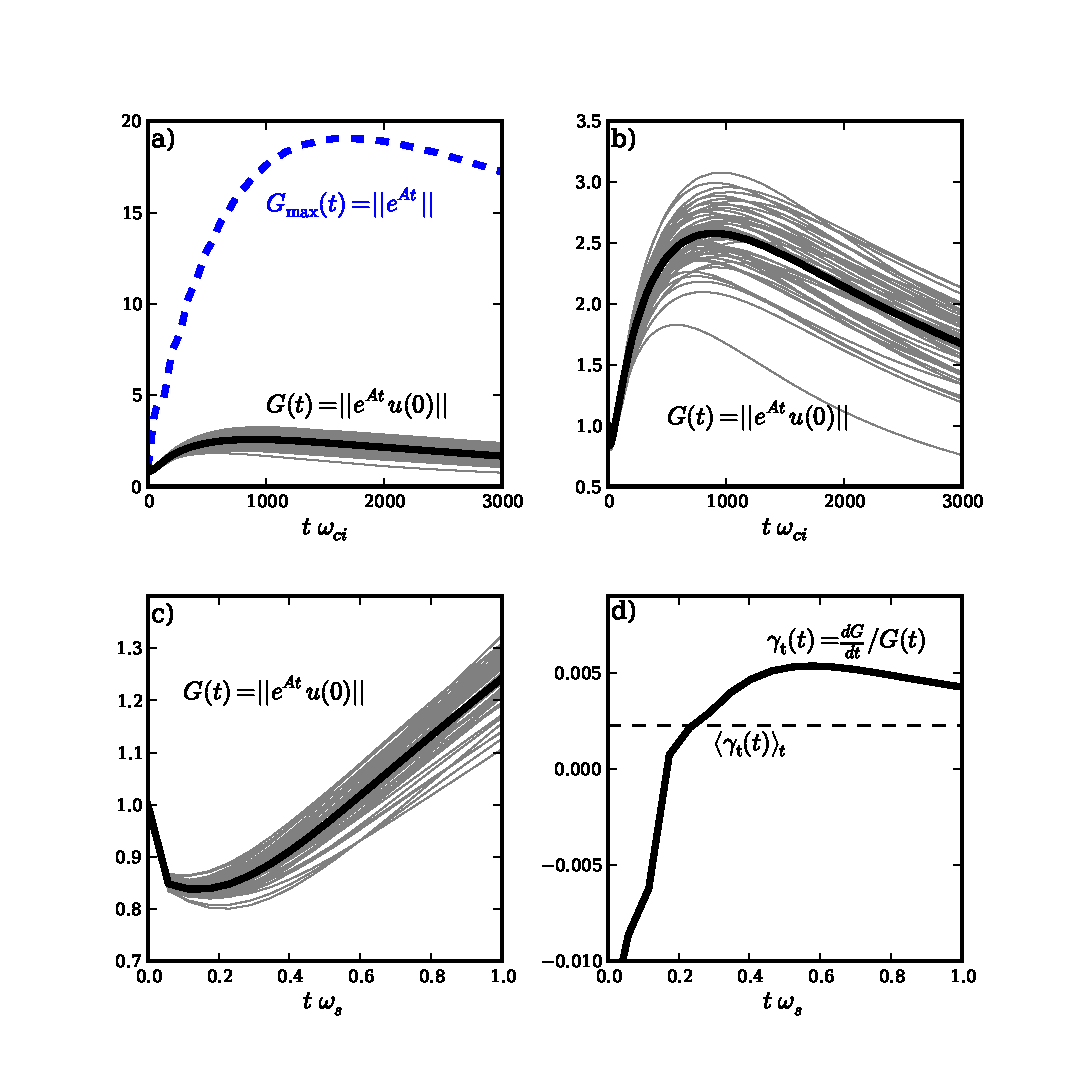
\includegraphics[]{m20n0_time_evs}}
\caption{a) The maximum growth ratio curve $G_{\rm{max}}(t)$ (dashed line) for $n=0,m=20$, and an ensemble of growth ratio curves (solid gray lines, with the solid black line the ensemble average)
that start with a random initial condition $u(0)$ and evolve under the linear operator. b) A zoomed in version of the ensemble of growth ratio curves. c) A further zoomed in version of the ensemble of
curves with a time range of $\omega_s^{-1}$, which is the characteristic linear time scale for drift waves. 
d) The instantaneous growth rate as a function of time of the the ensemble averaged growth ratio along with the average value over the time spanning $\omega_s^{-1}$.}
\label{m20n0_time_evs}
\end{figure}

It is not surprising that non-modal analysis has remained a qualitative endeavor due to its intrinsic dependence on initial conditions and the time-dependent growth properties of initial-value analysis.
The key to quantifying non-modal analysis and making it predictive is to successfully model the effect that the nonlinearities have on the transient linear processes.
In this regard, we model the nonlinearities as a periodic randomizing force. That is, the nonlinearities randomize the turbulent spatial structures on a characteristic nonlinear time scale. 
In practice, we completely randomize the system (initial condition) and then let it evolve linearly for a time $t_{nl}$, at which point, the system is re-randomized.
While the nonlinearities obviously do not affect the system in discrete time steps, this simplification provides a way to use linear non-modal analysis in a predictive manner. 
Since we do not know, \emph{a priori} at what level the turbulence will saturate, 
we cannot calculate the relative magnitude of the nonlinear terms in the equations to get the nonlinear time scale $t_{nl}$.
Thus, we invoke the conjecture of \emph{critical balance}, which posits that the nonlinear time scale equals the linear time scale at all spatial scales~\cite{schekochihin2012}. 
We can then estimate the nonlinear time scale as $t_{nl} = \omega_s^{-1}$, the inverse of the linear frequency of the fastest growing linear eigenmode (at each $m,n$).

In Fig.~\ref{m20n0_time_evs} c), we show the randomly initialized linear evolution curves from start up until a time of $\omega_s^{-1}$. 
Then, in Fig.~\ref{m20n0_time_evs} d), we calculate the instantaneous growth rate as a function of time of the ensemble averaged curve over that time period. 
For comparison, the instantaneous growth rate of the maximum growth curve is also shown.
In theory, this method should produce ensembled-averaged growth rate curves (like that in Fig.~\ref{m20n0_time_evs} d)) that have instantaneous growth rates consistent with the instantaneous
turbulent growth rates. Both the instantaneous transient growth rates and the turbulent growth rates have an average and a range associated with them. We show a comparison of their averages
in Fig.~\ref{spec_nl_transient_gamma}, which we call the Transient and Turbulent Growth Rate Spectra. The $n=0$ curves are fairly similar, especially when compared to the eigenmode spectra, also
shown in Fig.~\ref{spec_nl_transient_gamma}, although the transient curve is slightly down-shifted in $m$ compared to the turbulent curve. 
The $n=1$ curves, on the other hand, are not very similar, although they trend with $m$ in the same way, which is very different from the linear eigenmode trend.
The difference between the $n=1$ transient and turbulent growth rate spectra is due to nonlinear effects not captured by the simple transient calculation procedure. In particular, the turbulence
exhibits strong energy transfer from $n=0$ to $n=1$ Fourier components which is then dissipated by electron-ion collisions as the electrons stream along the field lines~\cite{friedman2012b}. 
This extra $n=1$ energy dissipation in the turbulent simulation is not a transient effect, and the $n=0$ to $n=1$ transfer is not a simple nonlinear mixing effect.

\begin{figure}
\centerline{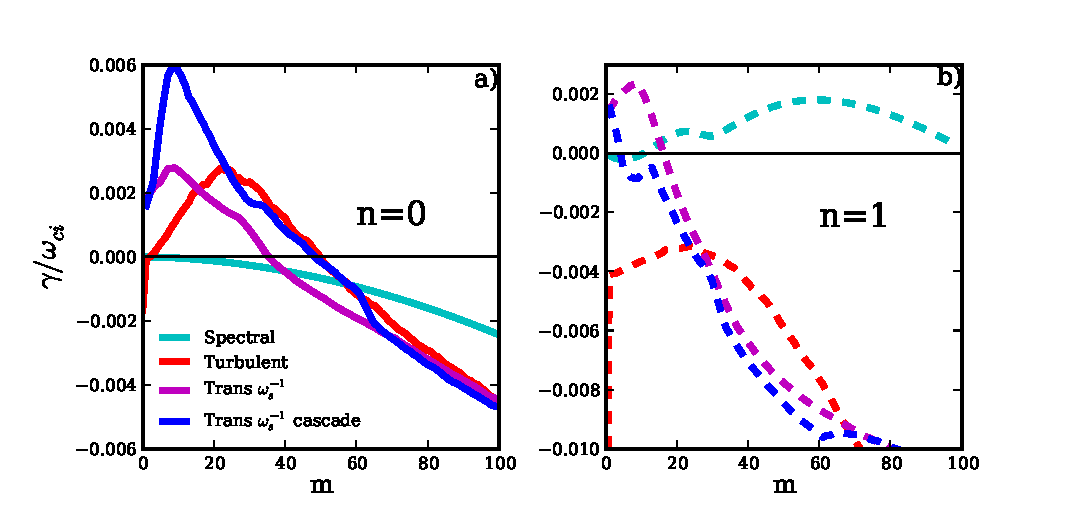
\includegraphics[]{spec_nl_transient_gamma}}
\caption{The linear, turbulent, and transient growth rate spectra. The transient growth rate spectra is calculated by the average growth rate over a time $\omega_s^{-1}$ for the ensemble average
growth ratio curves.}
\label{spec_nl_transient_gamma}
\end{figure}

Nevertheless, our randomizing transient method, which requires only linear calculations, reproduces energetic growth properties of the turbulence that are not captured by eigenmode analysis.
Clearly, when the linear systems are highly non-normal, transient growth rate analyses should be performed in place of (or in addition to) linear eigenmode analyses. 
Furthermore, the transient growth rates should be used in the kinds of predictions that are currently made with eigenmode growth rates. 
For instance, quasilinear theory uses the most unstable eigenmode growth rate $\gamma_{s,max}$ to predict the turbulent saturation levels through the mixing length formula $\gamma/k_\perp^2$. 
Using this formula with $\gamma_{s,\rm{max}} = 0.002$ and $m=60$, one would predict a turbulent saturation level on the order of $0.1 \%$. 
On the other hand, using this formula with the transient values -- $\gamma_{t,\rm{max}} = 0.003, m=10$ -- we predict the saturation level on the order of $10 \%$,
which matches the saturation level in the nonlinear simulation.

In summary, non-modal linear calculations are more informative than normal mode calculations when the linear system under consideration is highly non-normal. In the specific case of a low-flow
LAPD experiment, a nonlinear instability with linear $k_\para=0$ drive dominates the energy dynamics of the turbulence. While this is a surprising result in light of normal mode analysis,
it is not at all surprising given the system's non-modal behavior. In general, non-modal initial-value analysis is difficult to quantify and make predictive, but using some simple nonlinear modelling,
we have shown that it is possible.

\begin{acknowledgments}

\end{acknowledgments}


%%%%%%%%%%%%%%%%%%%%%%%%%%%%%%%%%%%%%%%%%%%%%%%%%%%%%%%%%%%%%%%%%%%%%%%%%%%


\bibliography{refs}
%\bibliographystyle{unsrt}


\end{document}
